\section{Аннотация[TODO]}
Гипероктаэдральные или кубические комбинаторные виды --- развитие идеи
комбинаторных типов (species). Мы будем обозначать их h-species для
краткости.
В работе частично разработан комбинаторный язык для h-species.
Написана формула для композиции цикленных индексов. Рассмотрены примеры.

\section{Введение}

\subsection{Комбинаторные виды}
Комбинаторные виды (\emph{species}) были введены Джоялем в [ref, ref, ref].
Они, в некоторой степени, являются развитием идеи производящих функций.
О комбинаторных видах можно говорить на нескольких языках: категорном,
комбинаторном и на языке теории представлений. Последний наиболее часто
встречается в литературе, хотя автору он кажется наимение выразительным.
Во введении изложено начало теории комбинаторных видов.
\subsubsection{Определение}
Рассмотрим категорию $\B$ --- подкатегорию конечных множеств с
морфизмами --- только биекциями. Это подкатегория в $\Set$. Функтор
$F:\B \rightarrow \Set$~--- это комбинаторный вид. То есть вид, это
сопоставление каждому числу $n \in \mathbb N$ множества с действием группы
$S_n$. Комбинаторная интерпретация: множеству точек сопоставляется
множество структур на этих точках, а действие $S_n$ ествественно возникает из
перестановок исходных точек. 
\begin{example}
Вид $\mathbb E$ --- структура множеста. Он
сопоставляет набору точек одно множество, состоящие из этих точек. Все элементы $S_n$
переходят в тождественное отображение. 
\end{example}
\begin{example}
$\mathbb C$ --- циклический порядок. Сопоставляет набору из $n$ точек $(n-1)!$
возможных циклических порядков на них. 
\end{example}
\begin{example}
Линейный порядок $\mathbb L$ сопоставляет $n!$ линейных
порядков. 
\end{example}
\begin{example}
$\mathbb E_e$ --- сужение $\mathbb E$ на четные множества. То есть для четных
$n$, совпадает с $\mathbb E$, а для нечетных $\emptyset$. Аналогично $\mathbb
E_o$ --- сужение на нечетные.
\end{example}
\begin{example}
На картинке \ref{pic:3-rooted-trees} изображен вид <<корневые
деревья с 3 вершинами>> (без какого-либо порядка на потомках).
\end{example}

\begin{figure}
\begin{center}
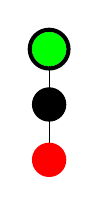
\begin{tikzpicture}
\draw (0pt, 0pt) -- (0pt, -20pt);
\draw (0pt, -20pt) -- (0pt, -40pt);
\draw[color=green, fill] (0pt,0pt) circle (6pt);
\draw[color=black, line width=1.5pt] (0pt,0pt) circle (7pt);
\draw[color=black, fill] (0pt, -20pt) circle (6pt);
\draw[color=red, fill] (0pt, -40pt) circle (6pt);
\end{tikzpicture}
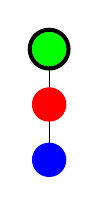
\begin{tikzpicture}
\draw (0pt, 0pt) -- (0pt, -20pt);
\draw (0pt, -20pt) -- (0pt, -40pt);
\draw[color=green, fill] (0pt,0pt) circle (6pt);
\draw[color=black, line width=1.5pt] (0pt,0pt) circle (7pt);
\draw[color=red, fill] (0pt, -20pt) circle (6pt);
\draw[color=blue, fill] (0pt, -40pt) circle (6pt);
\end{tikzpicture}
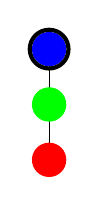
\begin{tikzpicture}
\draw (0pt, 0pt) -- (0pt, -20pt);
\draw (0pt, -20pt) -- (0pt, -40pt);
\draw[color=blue, fill] (0pt,0pt) circle (6pt);
\draw[color=black, line width=1.5pt] (0pt,0pt) circle (7pt);
\draw[color=green, fill] (0pt, -20pt) circle (6pt);
\draw[color=red, fill] (0pt, -40pt) circle (6pt);
\end{tikzpicture}
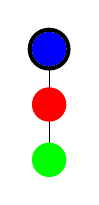
\begin{tikzpicture}
\draw (0pt, 0pt) -- (0pt, -20pt);
\draw (0pt, -20pt) -- (0pt, -40pt);
\draw[color=blue, fill] (0pt,0pt) circle (6pt);
\draw[color=black, line width=1.5pt] (0pt,0pt) circle (7pt);
\draw[color=red, fill] (0pt, -20pt) circle (6pt);
\draw[color=green, fill] (0pt, -40pt) circle (6pt);
\end{tikzpicture}
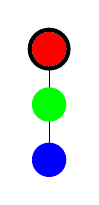
\begin{tikzpicture}
\draw (0pt, 0pt) -- (0pt, -20pt);
\draw (0pt, -20pt) -- (0pt, -40pt);
\draw[color=red, fill] (0pt,0pt) circle (6pt);
\draw[color=black, line width=1.5pt] (0pt,0pt) circle (7pt);
\draw[color=green, fill] (0pt, -20pt) circle (6pt);
\draw[color=blue, fill] (0pt, -40pt) circle (6pt);
\end{tikzpicture}
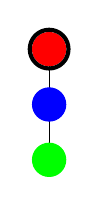
\begin{tikzpicture}
\draw (0pt, 0pt) -- (0pt, -20pt);
\draw (0pt, -20pt) -- (0pt, -40pt);
\draw[color=red, fill] (0pt,0pt) circle (6pt);
\draw[color=black, line width=1.5pt] (0pt,0pt) circle (7pt);
\draw[color=blue, fill] (0pt, -20pt) circle (6pt);
\draw[color=green, fill] (0pt, -40pt) circle (6pt);
\end{tikzpicture}
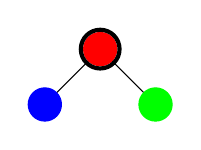
\begin{tikzpicture}
\draw (0pt, 0pt) -- (-20pt, -20pt);
\draw (0pt, 0pt) -- (20pt, -20pt);
\draw[color=red, fill] (0pt,0pt) circle (6pt);
\draw[color=black, line width=1.5pt] (0pt,0pt) circle (7pt);
\draw[color=blue, fill] (-20pt, -20pt) circle (6pt);
\draw[color=green, fill] (20pt, -20pt) circle (6pt);
\end{tikzpicture}
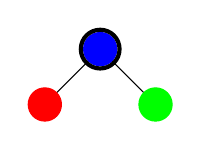
\begin{tikzpicture}
\draw (0pt, 0pt) -- (-20pt, -20pt);
\draw (0pt, 0pt) -- (20pt, -20pt);
\draw[color=blue, fill] (0pt,0pt) circle (6pt);
\draw[color=black, line width=1.5pt] (0pt,0pt) circle (7pt);
\draw[color=red, fill] (-20pt, -20pt) circle (6pt);
\draw[color=green, fill] (20pt, -20pt) circle (6pt);
\end{tikzpicture}
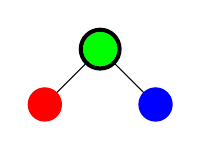
\begin{tikzpicture}
\draw (0pt, 0pt) -- (-20pt, -20pt);
\draw (0pt, 0pt) -- (20pt, -20pt);
\draw[color=green, fill] (0pt,0pt) circle (6pt);
\draw[color=black, line width=1.5pt] (0pt,0pt) circle (7pt);
\draw[color=red, fill] (-20pt, -20pt) circle (6pt);
\draw[color=blue, fill] (20pt, -20pt) circle (6pt);
\end{tikzpicture}
\end{center}
\caption{корневые деревья с 3 вершинами}
\label{pic:3-rooted-trees}
\end{figure}

Можно рассмотреть функтор $I:\Set \rightarrow Vec$, который сопоставляет множеству
векторное пространство со свободным[так можно сказать?] базисом из этого
множества.
Тогда $F \circ I: \B \rightarrow Vec$, получается для каждого $n$
перестановочное представление группы $S_n$. При таком подходе, характер этого
представления $\chi(\sigma)$, это количество структур, неподвижных относительно $\sigma \in S_n$.

\subsubsection{Сложение комбинаторных видов}
Сумму двух species $F, G$ легко определить как поточечную сумму функторов [ref].
На комбинаторном языке это будет означать <<либо структура типа $F$, либо
структура типа $G$>>. 
\begin{example}
$\mathbb E = \mathbb E_e + \mathbb E_o$
\end{example}
\begin{example}
Любой вид $F$ можно разложить в такую сумму $F =
F_{1} + F_{2} + F_{3} + \dots$, где $F_{i}$ --- сужение $F$ на $i \in \mathcal
B$. Значение $F_{i}$ на $j \neq i$ равно $\emptyset$.
\end{example}

\subsubsection{Произведение комбинаторных видов[TODO: тут какая-то чушь
написана, надо переписать]} Для определения произведения, используется тензорное
произведение на $\mathcal B$: $n \otimes m = (n + m)$ и соответствующее ему вложение $S_n \times S_m
\hookrightarrow S_{n+m}$. Все такие вложения сопряжены. На языке представлений
это соответствует индуцированному представлению $F(S_n \times S_m)\uparrow =
F(S_{n+m})$. [ref]

Поскольку $F_i \times G_j = (F \times G)_{i+j}$, то в целом произведение
соответствует свертке: $(F \times G)[n] = \sum\limits_{i=0}^{n}F[i] \times
G[i]$. На комбинаторном языке это значит: разбить множество точек на два кусочка
(на всевозможные размеры) и на первом ввести структуру типа $F$, на втором ---
типа $G$.
\begin{example}
$\mathbb E \times \mathbb E_1$ --- множество с выделенной точкой.
\end{example}
\begin{example}
$\mathbb C^2$ --- (упорядоченная) пара циклов.
\end{example}

\subsection{Композиция комбинаторных видов}
Кроме сложения и умножения на species можно ввести операцию композиции. Для
этого необходимо ввести дополнительную конструкцию: аналитический функтор.
\subsubsection{Аналитический функтор комбинаторных видов}
Аналитический функтор $\mathcal F$ соответствующий species $F$ является
продуктивной конструкцией, позволяющей определить композиционное произведение
species. Вводить его можно разными способами, мы ограничимся универсальным
свойством и явной конструкцией. Аналитический функтор является левым расширением по Кану функтора $F$
относительно $i$.

\begin{tikzpicture}
\label{comm:an}
	\node (B) {$\B$};
	\node (S1) [below of=B] {$\Set$};
	\node (S2) [right of=B, node distance=3cm] {$\Set$};
	\draw [right hook->] (B) to node [swap] {$i$} (S1);
	\draw [->] (B) to node {$F$} (S2);
	\draw [->] (S1) to node [swap] {$\mathcal F$} (S2);	
\end{tikzpicture}

Эта диаграмма не является коммутативной, а коммутативна лишь настолько, насколько может быть коммутативной диаграмма
подобного вида. А именно, имеется  естественное преобразование  $\kappa \colon
F \rightarrow i \circ \mathcal F$, обладающее следующим универсальным свойством:
 для любого функтора $M \colon
\Set \rightarrow \Set$ и морфизма функторов $\eta \colon F \rightarrow i \circ M$
этот морфизм пропускаеться через $\mathcal F$ при помощи $\kappa$.

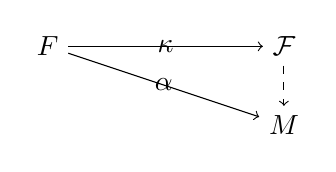
\begin{tikzpicture}
\label{comm:an-uni}
	\node (F) {$F$};
	\node (Fm) [right of=F, node distance=3cm] {$\mathcal F$};
	\node (M) [below of=Fm] {$M$};
	\draw [->] (F) to node {$\kappa$} (Fm);
	\draw [->] (F) to node [swap] {$\alpha$} (M);
	\draw [->, dashed] (Fm) to node [swap] {} (M);
\end{tikzpicture}


Явная конструкция для аналитического функтора. Для доказательства см (TODO)
\begin{equation}
\label{eq:an}
	\mathcal F(A) = \sum\limits_n F[n] \times A^n / S_n
\end{equation}

У аналитического функтора для типа структуры $F$ имеется прозрачный комбинаторная интерпретация.
Если трактовать множество $A$ как набор цветов,
то значение аналитического функтора $\mathcal F(A)$ трактуется как множество структур типа $F$
раскрашенных в цвета из $A$.

\subsubsection{Композиция аналитических функторов комбинаторных видов}
\begin{theorem}
Композиция аналитических функторов $\mathcal F \circ \mathcal G$ является
аналитическим функтором.
\end{theorem}
\begin{proof}
Species, которому соответствует этот аналитический функтор будем называть
композицией $F \circ G$.
Дадим набросок доказательства. Согласно конструкции $(\mathcal F \circ \mathcal
G) (A) = \sum\limits_n F[n] \times (\sum\limits_m G[m] \times A^m / S_m)^n /
S_n = \sum\limits_n \sum\limits_{k, m_1 + \dots + m_k = n} F[k] \times
(\coprod\limits_{i} G[m_i]) \times A^n / S_n$. [TODO??]

Строгое доказательство см. в [ref]
\end{proof}
Надо отметить, что все части разбиения предполагаются непустыми, что равносильно
сужению внутреннего speceis на $\mathbb N_{+}$. Будем обозначать его $G_{+}$.

У этого определения есть простая, наглядная
комбинаторная интерпретация: каждую точку структуры $F$ раздуваем(красим) в
структуру типа $G$.
\begin{example}
$\mathbb E_1 \circ F_{+} = F_{+}$, $F \circ \mathbb E_1 = F$. $\mathbb E_1$
является нейтральным элементом в монойде species по композиции.
\end{example}
\begin{example}
$\mathbb E_2 \circ \mathbb C$ --- (неупорядоченная) пара циклов.
\end{example}
\begin{example}
$\mathbb E \circ \mathbb E_{+}$ --- структура разбиения множества. Здесь $E_{+}$
--- непустые множества.
\end{example}
\begin{example}
$\mathbb E \circ \mathbb C_{+} = \mathbb S$ --- структура перестановки.
Буквально перестановка --- это набор непустых циклов.
\end{example}

В дальнейшем мы зачастую будем опускать $F \circ G_{+}$ и писать просто $F
\circ G$.

\subsubsection{Цикленный индекс}
Процедура декатегорификации не имеет строго математического смысла, так же как и процедура квантования.
Сейчас мы предложим процедуру, которая, стартуя с обычных species,
на выходе дает классический цикленный индекс/фробениусову характеристику.
Затем мы попытаемся аналогические действия провести и в гипероктаэдральном случае.
Декатегорификацией моноидальной категории $\mathbb B$ является моноид классов изоморфизма объектов категории
$\mathbb \B$, то есть моноид натуральных чисел по сложению.
Декатегорификкацией $\widehat{\mathbb \B}$ естественным образом оказывается
моноидная алгебра с коэффициентами из $\mathbb Z$ для моноида $\mathbb N$, то есть кольцо многочленов $Z[X]$.
(Правда это не то, что мы хотели. Чтобы получить цикленный индекс надо декатегорифицировать
саму операцию подстановки и аналитический функтор). [TODO: этот таинственный
абзац стоит переписать]

Надо устроить морфизм из моноидальной
категории (категории с тензорным произведением) в какую-нибудь алгебру функций. Мы вводим весовую
функцию таким образом что орбита раскрашенной структуры под действием $S_n$ имеет один и тот же вес.
После этого можно задать вопрос о коэффициенте при мономе соответствующего веса.
Это будет число орбит с заданной весовой функцией. По Лемме Бернсайда это то же
самое, что и усредненное число неподвижных точек по всем элементам группы. Чтобы
раскрашенная структура была неподвижна под действием перестановки $\sigma$
нужно, чтобы во-первых она была неподвижна как нераскрашенная структура, а
во-вторых расскраска должна переходить в себя. В качестве
весовой функции выбираем моном возникающий в произведении переменных отвечающим
цветам. Например расскраске в которой 2 первых цвета и 1 второй
соответсвует моном $x_1^2x_2$. Тогда первое условие дает нам сомножитель
$\chi(\sigma)$, где характер это характер соответствующего перестановочного
представления с базисом из структур. Второе условие требует покраски каждого
цикла в один и тот же цвет. Итоговая формула называеться фробениусовой
характеристикой / цикленным индексом. Она считает количество неподвижных
раскрашенных структур в среднем. 

\begin{equation}
\label{eq:fr}
\mathcal Z_F =
\sum_{n}\frac{1}{n!}\sum_{\sigma \in S_n}\chi(\sigma)\psi^{\lambda(\sigma)} =
\sum_{n, \lambda \vdash n}\chi(\sigma_{\lambda})
\frac{\psi^{\lambda}}{z_{\lambda}}
\end{equation}

Где $\chi$ --- характер (перестановочного) представления заданного $F$, $\sigma$
--- перестановка цикленного типа $\lambda$, 
$\psi^{\lambda} = 
(x_1^{\lambda_1} + x_2^{\lambda_1} + x_3^{\lambda_1} + \dots)
(x_1^{\lambda_2} + x_2^{\lambda_2} + x_3^{\lambda_2} + \dots)
(x_1^{\lambda_3} + x_2^{\lambda_3} + x_3^{\lambda_3} + \dots)
\dots$,
 $z_\lambda$ --- индекс класса сопряженности $\sigma$.
Появляется она из следующих соображений: в числителе стоит симметрическая
функция считающая все неподвижные раскраски. Цвета это $x_1, x_2, x_3, \dots$

\begin{example}
$\mathcal Z_{\mathbb E} = e^{(\psi^1 + \frac{\psi^2}{2} + \frac{\psi^3}{3} +
\dots)}$. Для доказательства смотри [ref].
\end{example}

\subsubsection{Плетизм цикленных индексов}
\begin{theorem}
Композиции аналитически функторов соответствует плетизм цикленных
индексов.
\end{theorem}
Чудесный факт заключается в том, что в декатегорификации
композиция соответствует простой формуле подстановки. Сейчас мы ее напишем и
приведем набросок доказательства. В качестве множества цветов $A$ рассмотрим
счетный набор цветов $x_1, x_2, x_3, \dots$ Цикленный индекс запишем
относительно базиса кольца симметрических функций $\psi^1, \psi^2, \psi^3, \dots$
\begin{multline}
\label{eq:zfg}
	\mathcal Z_{F \circ G} (\psi^1, \psi^2, \psi^3, \dots) = \\
	\mathcal Z_F(
		\mathcal Z_G(\psi^1, \psi^2, \psi^3, \dots),
		\mathcal Z_G(\psi^2, \psi^4, \psi^6, \dots),
		\mathcal Z_G(\psi^3, \psi^6, \psi^9, \dots),
		\dots
	)
\end{multline}

В композиции двух аналитических функторов получается, что цвета в которые мы
красим структуру $F$ это структуры типа $G$. То есть $\mathcal Z_{F \circ G} =
\mathcal Z_F(\psi_g^1, \psi_g^2, \psi_g^3, \dots)$, где $\psi_g^i = (g_1^i +
g_2^i + g_3^i + \dots)$, где $g_i$ --- перечисление всех структур типа $G$.
Нужно раскрыть переменные $g_i $ --- написать их относительно начальных цветов.
Формулу $\psi_g^i = \mathcal Z_G(\psi^i, \psi^{2i}, \psi^{3i}, \dots)$ легко
понять в переменных $x_1, x_2, x_3, \dots$. Мы должны покрасить $i$ кусков в
одну и ту же $G$--структуру. Значит каждый цвет $x_j$ заменяется на $x_j^i$.

Формулу \ref{eq:zfg} можно специализировать для подсчета labeled--структур. То
есть покрашенных структур у которых нет двух одинаковых цветов в расскраске.
Соответсвующие мономы (в базисе $x_1, x_2, x_3, \dots$) возникают только при
раскрытии мономов вида $c(\psi^1)^k$ и коэффициент в них равен $ck!$ --- такой
же как при мономе с точностью до факториала. Этот факториал приводит к
необходимости рассматривать экспоненциальные производящие функции вместо
обычных. Можно занулить все остальные мономы подстановкой $\psi^1 = t, \psi^2 =
0, \psi^3 = 0, \psi^4 = 0$. Формула \ref{eq:zfg} примет вид $
\mathcal Z_{F \circ G} (t, 0, 0, \dots) =
	\mathcal Z_F(
		\mathcal Z_G(t, 0, 0, \dots), 0, 0, \dots
	)
$.
А значит для экспоненциальных производящих функции labeled-структур справедливо
равенство
\begin{equation}
\label{eq:comp}
(f \circ g) (t) = f(g(t))
\end{equation}

\begin{example}
(Экспоненциальная) производящая функция для $\mathbb E$ это $e^x = 1 + x +
\frac{1}{2!}x^2 + \frac{1}{3!}x^3 + \dots$. А производящая функция для
непустых циклов $\mathbb C_{+}$ это $-log(1-x) = x + \frac{1}{2}x^2 +
\frac{1}{3}x^3 + \dots$.
А для $\mathbb S$ производящая функция это $\frac{1}{1-x} = 1 + x + x^2 + x^3 +
\dots$.
И действительно $e^(-log(1-x)) = \frac{1}{1-x}$.
\end{example}
